\documentclass[10pt,a4paper]{article}
\usepackage[utf8]{inputenc}
\usepackage{amsmath}
\usepackage{amsfonts}
\usepackage{amssymb}
\usepackage{graphicx}
\usepackage{verbatim}
\usepackage[margin=1in]{geometry}

\setlength\parindent{0pt} % Removes all indentation from paragraphs

\author{Nikola Janju\v{s}evi\'{c}}
\title{ECE471, Selected Topics in Machine Learning \\ Assignment 1}
\date{September 11, 2018}

\begin{document}
\begin{large}
ECE471, Selected Topics in Machine Learning -- Assignment 1
\end{large} \\
Nikola Janju\v{s}evi\'{c} \\
September 11th 2018


\begin{verbatim}
#!/bin/python3.6
import matplotlib.pyplot as plt
import numpy as np
import tensorflow as tf
import time

from tqdm import tqdm

NUM_FUNCTIONS = 10
BATCH_SIZE = 50
NUM_BATCHES = 300

class Data(object):
    def __init__(self):
        num_samp = 50
        sigma = .1
        np.random.seed(int(time.time()))

        self.index = np.arange(num_samp)
        self.x = np.random.uniform(size=(num_samp))
        self.y = np.sin(2*np.pi*self.x) + \
            sigma*np.random.normal(size=self.x.shape)

    def get_batch(self):
        choices = np.random.choice(self.index, size=BATCH_SIZE)
        return self.x[choices], self.y[choices].flatten()

def f(x):
    w  = tf.get_variable('w', [NUM_FUNCTIONS, 1], tf.float32,
                        tf.random_normal_initializer())
    mu =  tf.get_variable('mu', [NUM_FUNCTIONS, 1], tf.float32,
                        tf.random_normal_initializer())
    sig = tf.get_variable('sig', [NUM_FUNCTIONS, 1], tf.float32,
                        tf.random_normal_initializer())
    b  = tf.get_variable('b', [], tf.float32, tf.zeros_initializer())

    return tf.squeeze(tf.matmul(tf.exp(-tf.pow((x-mu)/sig,2)),
        w, transpose_a=True) + b)


x = tf.placeholder(tf.float32, [BATCH_SIZE])
y = tf.placeholder(tf.float32, [BATCH_SIZE])
y_hat = f(x)

loss = tf.reduce_mean(tf.pow(y_hat - y, 2))
optim = tf.train.GradientDescentOptimizer(learning_rate=0.1).minimize(loss)
init = tf.global_variables_initializer()

sess = tf.Session()
sess.run(init)

data = Data()

for _ in tqdm(range(0, NUM_BATCHES)):
    x_np, y_np = data.get_batch()
    loss_np, _ = sess.run([loss, optim], feed_dict={x: x_np, y: y_np})

w, mu, sig, b = [np.array(sess.run(var)) for var in
    tf.get_collection(tf.GraphKeys.TRAINABLE_VARIABLES)]

# plotting
xx = np.linspace(-.1,1.1,1000)
xx = xx.reshape((len(xx),1)).T
# model
yy = np.matmul(np.exp(-((xx-mu)/sig)**2).T, w) + b

fig, (ax1,ax2) = plt.subplots(1,2)
# FIT PLOT
ax1.set_title("Fit")
# sine wave
ax1.plot(xx.T,np.sin(2*np.pi*xx.T))
# model
ax1.plot(xx.T,yy,'r',linestyle="dashed")
# noisey sine wave
ax1.plot(data.x,data.y,'og',ms=4,markeredgecolor="black")
ax1.set_xlim(-.1,1.1)
ax1.set_xlabel("x")
ax1.set_ylabel("y")
ax1.legend(["Sine-Wave","Model","Noisey Sine-Wave ($\sigma_n = 0.1$)"])

# BASES FUNCTION PLOT
for i in range(len(w)):
    ax2.plot(xx.T,np.exp(-((xx-mu[i])/sig[i])**2).T)
ax2.set_title("Bases Functions: "
    r"$\phi_i(x) = e^{(x-\mu_i)^2/\sigma_i^2}$")
ax2.set_xlim(-.1,1.1)
ax2.set_xlabel("x")
ax2.set_ylabel("y")
plt.show()
\end{verbatim}

\begin{figure}[h]
\centering
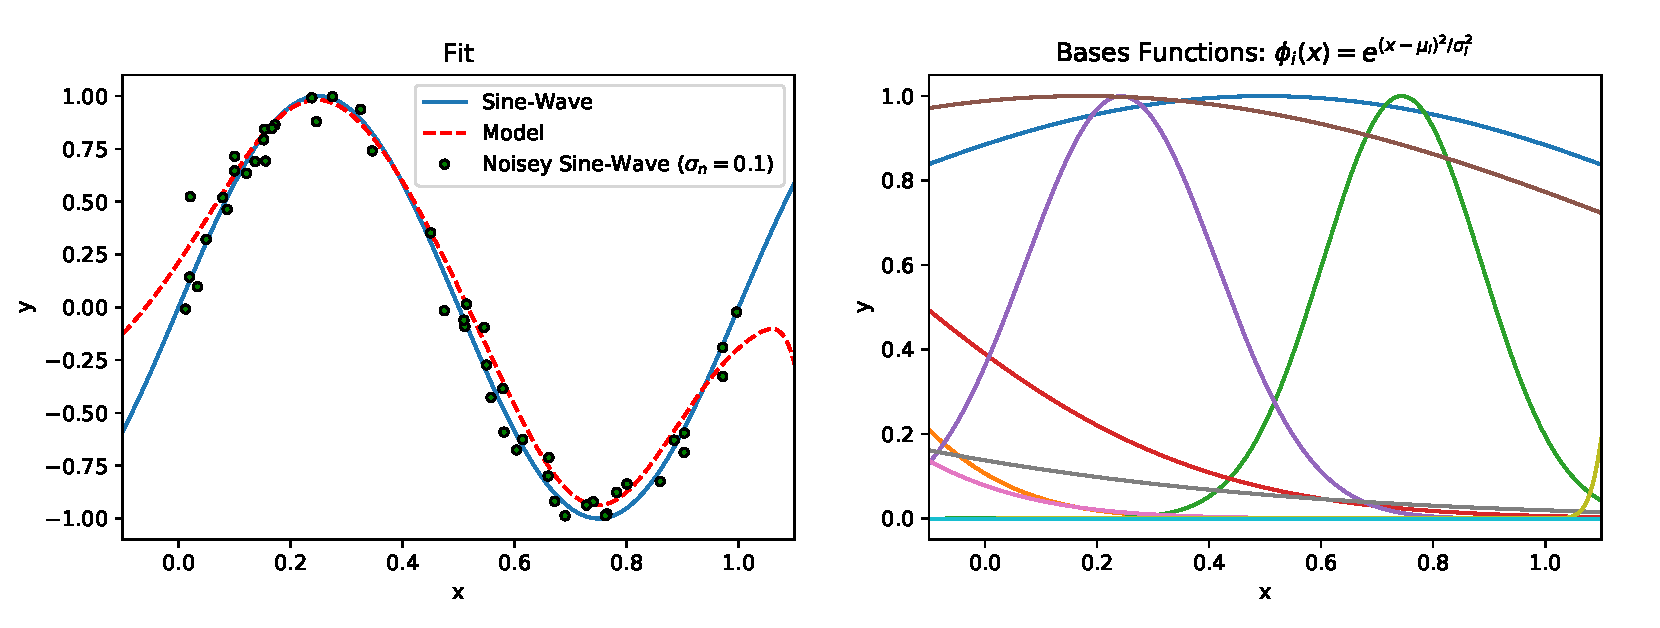
\includegraphics[width=\textwidth]{Figure_M10.pdf}
\caption{Model fit (left) and bases functions (right) for noisey sine-wave regression}
\end{figure}

\end{document}